\chapter{Uitwerking}
\label{ch:uitwerking}

Dit hoofdstuk bevat het onderzoek naar open source tools die in aanmerking komen als alternatief voor Fission. Er worden requirements vastgelegd in overleg met Nubera, op basis van deze requirements wordt een long list opgesteld met tools die in aanmerking komen. Na het evalueren van de long list worden de frameworks beoordeeld volgens het aantal requirements waaraan voldaan werd, het meest interessante framework vormt samen met Fission de shortlist. In de shortlist wordt dieper ingegaan op twee open source frameworks.

\section{Open Source tools}
Nubera heeft aangegeven op zoek te zijn naar open source serverless (FaaS) frameworks voor in house gebruik bij klanten. Met de term in house wordt de infrastructuur waarvan een organisatie gebruikmaakt geadresseerd, dit kan on-premises infrastructuur, een eigen datacenter of de private cloud betekenen. Nubera biedt momenteel nog geen serverless (FaaS) framework aan bij klanten. Voor Nubera is dit onderzoek zinvol zodat iedereen binnen Nubera een beeld heeft over wat serverless precies is, hoe dit kan worden opgezet en wat de technologie allemaal te bieden heeft. Enkele medewerkers binnen Nubera hebben al geëxperimenteerd met Fission, hiervoor bestaat reeds een interesse en daarom wil Nubera ook op zoek naar een alternatief dat dezelfde mogelijkheden (of meer) aanbiedt. De requirements waaraan de frameworks moeten voldoen worden opgelijst in volgende sectie. De opzet van deze studie maakt een vergelijking tussen twee open source frameworks die op basis van vooropgestelde requirements vergeleken worden. Het eerste framework dat sowieso opgenomen wordt in de Proof of Concept is Fission, een alternatief wordt gekozen na het uitwerken van de long list in overeenstemming met de vastgelegde requirements.

\section{Requirements analyse}
De requirements waaraan de FaaS frameworks moeten voldoen werden in overleg met Nubera gecapteerd. Er wordt een onderscheid gemaakt op basis van functionele en niet-functionele requirements, daarbinnen worden deze verder opgedeeld volgens de MoSCoW-techniek\footnote{https://bit.ly/2aecva4}. Binnen de twee grote requirements groeperingen worden de requirements opgesplitst in een ''Must-have'', ''Should-have'' en ''Nice-to-have'' klasse.

\subsection{Functionele requirements}
\subsubsection{Must-have}
\begin{itemize}
    \item Kubernetes als container orkestrator onderliggend.
    \item Ondersteund serverless functies in Python en Go.
    \item Functies zijn auto-scalable.
    \item Snelle uitvoeringstijd van functies: In de Proof of Concept zal de uitvoeringstijd van dezelfde functie die wordt uitgevoerd op beide frameworks worden gemeten. Op basis van de resultaten worden conclusies getrokken.
\end{itemize}
\subsubsection{Should-have}
\begin{itemize}
    \item Command line tools voor beheer van functies.
    \item Ondersteund serverless functies in Node.js.
    \item Deployment via Manifest op Kubernetes.
\end{itemize}
\subsubsection{Nice-to-have}
\begin{itemize}
    \item Ondersteund serverless functies in nog meer verschillende talen zodat hetzelfde framework kan gebruikt worden bij verschillende klanten.
    \item User interface voor beheer van functies.
\end{itemize}
\subsection{Niet-functionele requirements}
\subsubsection{Must-have}
\begin{itemize}
    \item Het framework moet open source zijn.
    \item Het framework moet gratis zijn.
    \item Minstens 40 ''contributors'' op GitHub.
    \item Minstens 3000 stars op GitHub. (Garantie voor populariteit in de community.)
    \item Gebruiksvriendelijk: De eigen ervaring wordt hier als norm genomen, op basis van het uitproberen en experimenteren wordt deze requirement gemeten.
    \item Eenvoudig op te zetten: Het installatieproces van het framework is goed gedocumenteerd en is eenvoudig te reproduceren.
\end{itemize}
\subsubsection{Should-have}
\begin{itemize}
    \item Enige maturiteit als garantie voor het functioneren van het framework. (Production ready)
    \item Contributors uit erkende organisaties.
    \item Het project wordt onderhouden, laatste commit is niet ouder dan 2 weken. (Datum van schrijven 13/04/2019)
    \item Goede en duidelijke documentatie.
\end{itemize}
\subsubsection{Nice-to-have}
\begin{itemize}
    \item Slack channel voor discussie over het framework.
\end{itemize}

\section{Long list}
De long list bevat alle mogelijke frameworks die in aanmerking komen overeenstemmend met de gecapteerde requirements. Elk framework wordt in het kort toegelicht. Na de oplijsting van de verschillende frameworks die in aanmerking komen worden er tabellen opgemaakt waarin terug te vinden is of de frameworks al dan niet aan de requirements voldoen, er is één tabel voor de functionele en één voor de niet-functionele requirements. Op basis van de tabellen wordt het meest veelbelovende framework gekozen dat zal worden vergeleken met Fission. De functionele en niet-functionele requirements worden per framework tegen elkaar afgewogen, executietijd van functies, gebruiksvriendelijkheid en eenvoud in installatie zijn niet meetbaar zonder Proof of Concept en zullen maar later in dit onderzoek worden gemeten. Deze requirements worden daarom ook niet in de tabellen opgenomen. De tabellen worden opgesteld aan de hand van onderzoek, er wordt op basis van gevonden resultaten een besluit gevormd, later kan dit echter wijzigen tijdens de Proof of Concept. Het is mogelijk dat ervan uitgegaan wordt tijdens het opstellen van de long list dat een framework voldoet aan een bepaalde requirement maar dat dit tijdens de opstelling in de Proof of Concept echter niet het geval blijkt.

\subsection{Fission}
Fission\footnote{https://fission.io/} is een serverless framework dat bovenop Kubernetes draait. Het stelt ontwikkelaars in staat functies te schrijven in verschillende programmeertalen. De functies kunnen eveneens worden gemapt aan HTTP triggers voor het aanroepen ervan.

\subsection{Kubeless}
Kubeless\footnote{https://kubeless.io/} is eveneens een Kubernetes native serverless framework dat ontwikkelaars in staat stelt kleine stukken code of functies op te laden zonder zorg over de onderliggende infrastructuur. Kubeless is de ideale tool voor ieder die op zoek is naar een open source alternatief voor wat AWS Lambda, Google Cloud Functions en Azure Functions aanbieden.

\subsection{OpenFaaS}
\textcite{OpenFaaS2019} beschrijft zichzelf als een framework voor het bouwen van serverless functies met Kubernetes en Docker, het voorziet ook support voor metrics. Tools als Prometheus kunnen makkelijk worden geïmplementeerd voor monitoring.

\subsection{Apache OpenWhisk}
OpenWhisk\footnote{https://openwhisk.apache.org/} is een open source serverless platform waar functies op gedeployed kunnen worden, gemapt aan events en triggers. OpenWhisk staat in voor het beheer van de hardware en schaalbaarheid van applicaties met behulp van Docker containers zodat ontwikkelaars zich kunnen focussen op het bouwen van applicaties.

\subsection{Fn}
De beschrijving waarmee \textcite{FnProject2019} zichzelf voorstelt luidt als volgt: ''Het Fn Project is een open source container-native serverless platform dat overal kan draaien, in elk type van cloud maar ook op locatie. Het is makkelijk in gebruik, ondersteund elke programmeertaal, is uitbreidbaar en performant.''

\subsection{IronFunctions}
Iron belooft met hun IronFunctions\footnote{https://open.iron.io/} serverless framework dat taken die veel CPU vragen onmerkbaar in de achtergrond draaien. Het laat ontwikkelaars toe functies te implementeren in applicaties en de focus te leggen op het schrijven van de software. Het voorziet ook snelle en eenvoudige configuratie van de onderliggende infrastructuur en job processing.

\subsection{OpenLambda}
OpenLambda\footnote{https://open-lambda.org/index.htm} is in tegenstelling tot de eerder besproken alternatieven minder ver ontwikkeld. OpenLambda is een framework dat interessant is voor iedereen die serverless wil testen leren kennen. OpenLambda is niet production ready, de eerder besproken tools zijn dit vaak wel al.

\subsection{Nuclio}
Nuclio\footnote{https://nuclio.io} wordt vaak gebruikt als alternatief voor AWS Lambda. Het is een serverless framework voor real-time functies en data gedreven applicaties. Nuclio draait eveneens bovenop Kubernetes.

\subsection{Knative}
Knative\footnote{https://pivotal.io/knative} is een uitbreiding van Kubernetes die helpt bij het bouwen van moderne, container-gebaseerde applicaties. Het is een open source project in samenwerking met Google. Knative voorziet ontwikkelaars dat ze op een eenvoudige manier applicaties bovenop een Kuberneteslaag kunnen draaien.

\subsection{Vergelijking}
In tabel \ref{tab:frameworks-fr} worden de verschillende frameworks vergeleken op basis van vooropgestelde functionele requirements.  De tabel duidt de requirements waaraan de frameworks voldoen aan met een ''X'', indien ze niet voldoen volgt er een ''-'' of aangepaste omschrijving. Tabel \ref{tab:frameworks-nfr} geeft een overzicht van de frameworks ten opzichte van de vooropgestelde niet-functionele requirements. In deze tabel geldt hetzelfde: een ''X'' wilt zeggen dat er aan de requirement is voldaan, een ''-'' betekent dat er een requirement niet voldaan is en een aangepaste beschrijving werd gekozen wanneer deze meer zegt dan een ''X'' of ''-''.


\begin{table}[]
    \centering
    \resizebox{\textwidth}{!}{%
        \begin{tabular}{llccccccccc}
            \hline
            \multicolumn{2}{l}{\textbf{}} & \multicolumn{1}{l}{\textbf{Fission}} & \textbf{Kubeless} & \textbf{OpenFaaS} & \textbf{OpenWhisk} & \textbf{Fn} & \textbf{IronFunctions} & \textbf{OpenLambda} & \textbf{Knative} & \textbf{Nuclio} \\ \hline
            \multirow{3}{*}{\textbf{Must-have}} & Kubernetes orkestratie & X & X & X & X & X & X & X & X & X \\
            & Python/Go support & X & X & X & X & X & X & Enkel Python & X & X \\
            & Autoscaling & X & X & X & X & X & - & - & X & X \\ \hline
            \multirow{3}{*}{\textbf{Should-have}} & Command line tools & X & X & X & X & X & X & - & X & X \\
            & Node.js support & X & X & X & X & X & X & - & X & X \\
            & Manifest deployment & X & X & X & X & - & - & - & X & X \\ \hline
            \multirow{2}{*}{\textbf{Nice-to-have}} & Support voor meer talen & X & X & X & X & X & X & - & X & X \\
            & User interface & X & X & X & - & X & X & - & X & X
        \end{tabular}%
    }
    \caption{Vergelijking open source serverless frameworks op basis van functionele requirements}
    \label{tab:frameworks-fr}
\end{table}


\begin{table}[]
    \centering
    \resizebox{\textwidth}{!}{%
        \begin{tabular}{llccccccccc}
            \hline
            \textbf{} &  & \textbf{Fission} & \textbf{Kubeless} & \textbf{OpenFaaS} & \textbf{OpenWhisk} & \textbf{Fn} & \textbf{IronFunctions} & \textbf{OpenLambda} & \textbf{Knative} & \textbf{Nuclio} \\ \hline
            \multirow{4}{*}{\textbf{Must-have}} & Open source & X & X & X & X & X & X & X & X & X \\
            & Gratis & X & X & X & X & X & X & X & X & X \\
            & \textgreater 40 contributors & 76 & 77 & 99 & 151 & 77 & 32 & 17 & 115 & 36 \\
            & \textgreater 3K GitHub stars & 4.2K & 4.5K & 13.8K & 3.9K & 3.9K & 2.5K & 593 & 1.6K & 2.6K \\ \hline
            \multirow{4}{*}{\textbf{Should-have}} & Maturiteit (Production ready) & X & X & X & X & X & - & - & X & X \\
            & Mede ontwikkeld door erkende organisaties & Platform9 & Bitnami & VMware & IBM & Oracle & iron.io & - & Google & - \\
            & Laatste commit (datum schrijven 13/04/2019) & 09/04/2019 & 09/04/2019 & 13/04/2019 & 11/04/2019 & 10/04/2019 & 20/08/2018 & 14/01/2019 & 13/03/2019 & 01/04/2019 \\
            & Goede/duidelijke documentatie & X & X & X & X & X & - & - & X & X \\ \hline
            \textbf{Nice-to-have} & Slack channel over het project & X & X & X & X & X & - & - & X & X \\ 
        \end{tabular}%
    }
    \caption{Vergelijking open source serverless frameworks op basis van niet-functionele requirements.}
    \label{tab:frameworks-nfr}
\end{table}

\subsubsection{Resultatenverwerking}
Op basis van tabel \ref{tab:frameworks-fr} worden eerst de functionele requirements vergeleken. Onmiddellijk is zichtbaar dat enkele frameworks minder interessant zijn dan anderen, zo voldoen IronFunctions en OpenLambda beiden niet aan de must-have requirements, daarom worden deze ook niet verder behandeld. Wanneer de should-have requirements in overweging worden genomen is duidelijk dat Fn geen deployment via Manifest voorziet en dus ook geen kanshebber meer is om vergeleken te worden met Fission. Alle frameworks behalve OpenWhisk voldoen aan de nice-to-have requirements. Er wordt besloten om enkel de frameworks te behandelen die voldoen aan alle voorgaande requirements. Momenteel bestaat de lijst van frameworks die in aanmerking komen nog uit: Kubeless, OpenFaaS, Knative en Fission. De niet-functionele requirements zullen doorslaggevend zijn in de keuze voor een alternatief FaaS framework.
\\\\
Tabel \ref{tab:frameworks-nfr} weergeeft dat alle frameworks voldoen aan de requirements open source en gratis. Wanneer er wordt gekeken naar het aantal contributors en het aantal ''stars'' op GitHub dan representeert dit de populariteit en de interesse voor het project binnen de community. Een hoger aantal contributors wijst vaak op meer kennis, meer review van code en enige zekerheid in vergelijking met een laag aantal contributors. De GitHub stars worden als factor gekozen om te meten hoe populair een framework is. De metingen werden gedaan op 13 april 2019 en kunnen tegen de tijd van lezen reeds gewijzigd zijn. Als norm werd vooropgesteld dat een project minstens veertig contributors moet hebben alsook een minimum van drieduizend stars. Van de overgebleven frameworks voldoet Knative niet aan het minimum aantal Github stars. Overige frameworks voldoen alleen aan de should-have requirements eveneens als de nice-to-have requirements. behalve Iron. Alle frameworks die resten zijn mede ontwikkeld door erkende organisaties, de bedrijven die werden opgelijst worden ook wel de ''backers'' van het project genoemd. De datum van de laatste commit is ook een belangrijk gegeven om te beslissen of het project overlevingskans heeft en up-to-date blijft. Alle overige projecten beschikken op het eerste zicht over duidelijke documentatie, al wordt dit pas duidelijk tijdens het uitwerken van de Proof of Concept. 

Tabel \ref{tab:frameworks-samenvattingl} weergeeft een samenvatting van de frameworks en het aantal requirements waaraan ze voldoen, de frameworks worden gerangschikt volgens de graad dat ze in aanmerking komen (van boven naar onder). In de tabel wordt telkens voor de verschillende categorieën van requirements een optelling gemaakt waaraan een framework voldoet. Uit de tabel is af te leiden dat OpenFaaS, Kubeless en Fission een maximumscore behalen. Na verder onderzoek werd besloten om verder te gaan met OpenFaaS als alternatief framework voor Fission. In sectie \ref{sec:short-list} worden Fission en OpenFaaS verder in detail besproken.Fission werd aangereikt door Nubera, als alternatief wordt OpenFaaS opgezet als vergelijking omdat dit uit het onderzoek naar de long list het meest veelbelovend blijkt. 
\\
\begin{table}[]
    \centering
    \resizebox{\textwidth}{!}{%
        \begin{tabular}{@{}llccccccccc@{}}
            \toprule
            &  & \multicolumn{3}{c}{\textbf{Functionele requirements}} & \textbf{} & \multicolumn{3}{c}{\textbf{Niet-functionele requirements}} & \textbf{} & \textbf{Totaal} \\ \midrule
            &  & \textbf{M-H} & \textbf{S-H} & \textbf{N-T-H} & \textbf{} & \textbf{M-H} & \textbf{S-H} & \textbf{N-T-H} & \textbf{} & \textbf{/17} \\
            \textbf{1.} & \textbf{OpenFaaS} & 3 & 3 & 2 &  & 4 & 4 & 1 &  & 17 \\
            \textbf{2.} & \textbf{Kubeless} & 3 & 3 & 2 &  & 4 & 4 & 1 &  & 17 \\
            \textbf{3.} & \textbf{Fission} & 3 & 3 & 2 &  & 4 & 4 & 1 &  & 17 \\
            \textbf{4.} & \textbf{OpenWhisk} & 3 & 3 & 1 &  & 4 & 4 & 1 &  & 16 \\
            \textbf{5.} & \textbf{Fn} & 3 & 2 & 2 &  & 4 & 4 & 1 &  & 16 \\
            \textbf{6.} & \textbf{Knative} & 3 & 3 & 2 &  & 3 & 3 & 1 &  & 15 \\
            \textbf{7.} & \textbf{Nuclio} & 3 & 3 & 2 &  & 2 & 3 & 1 &  & 14 \\
            \textbf{8.} & \textbf{IronFunctions} & 2 & 2 & 2 &  & 2 & 2 & 0 &  & 10 \\
            \textbf{9.} & \textbf{OpenLambda} & 1 & 0 & 0 &  & 2 & 0 & 0 &  & 3 \\
            &  & \multicolumn{1}{l}{} & \multicolumn{1}{l}{} & \multicolumn{1}{l}{} & \multicolumn{1}{l}{} & \multicolumn{1}{l}{} & \multicolumn{1}{l}{} & \multicolumn{1}{l}{} & \multicolumn{1}{l}{} & \multicolumn{1}{l}{} \\
            &  & \multicolumn{1}{l}{} & \multicolumn{1}{l}{} & \multicolumn{1}{l}{} & \multicolumn{1}{l}{} & \multicolumn{1}{l}{} & \multicolumn{1}{l}{} & \multicolumn{1}{l}{} & \multicolumn{1}{l}{} & \multicolumn{1}{l}{} \\ \bottomrule
        \end{tabular}%
    }
    \caption{Frameworks opgelijst in graad waarin ze in aanmerking komen. (M-H: Must-have, S-H: Should-have, N-T-H: Nice to have.) }
    \label{tab:frameworks-samenvattingl}
\end{table}

\section{Short List}
\label{sec:short-list}
Op basis van voorgaande long list worden, zoals eerder al aangehaald, Fission en OpenFaaS vergeleken. Nubera verwacht een framework dat in overeenstemming met opgestelde requirements een goed alternatief voor Fission kan bieden. De verdere uitwerking in de Proof of Concept tracht de requirments die nog niet werden gemeten te behandelen, dit zijn zowel functionele als niet-functionele requirements. In deze short list wordt dieper ingegaan op Fission en OpenFaaS, wat deze frameworks inhouden en aanbieden is terug te vinden in dit onderdeel.

\subsection{OpenFaaS}
OpenFaaS\footnote{https://www.openfaas.com/} is een open source Function as a Service (serverless) project dat werd opgestart door Alex Ellis. Alex is lid van het VMware Open Source Technology Center (OSTC), VMware is eveneens ''backer'' van dit project, ze ondersteunen in de ontwikkeling van OpenFaaS. Het project telt 13.8K GitHub stars, 99 contributors en is daarmee momenteel het grootste en populairste open source Function as a Service framework. OpenFaaS wordt al gebruikt bij verschillende grote organisaties zoals: VMware, BT (British Telecom), Citrix, Contiamo, University of Washington etc.
\\
De aspecten waarmee \textcite{OpenFaaS2019} uitpakt om zich te onderscheiden van anderen zijn:
\begin{itemize}
    \item Makkelijke installatie en eenvoud in gebruik door de beschikbare UI.
    \item Portable: draait op bestaande hardware of in de public/private cloud  bovenop Kubernetes of Docker Swarm.
    \item Functies in eender welke taal voor Linux of Windows.
    \item Auto-scalable wanneer de vraag verhoogt.
    \item YAML format voor templating en definiëren van functies.
\end{itemize}

\subsubsection{Architectuur}
OpenFaaS kan worden opgedeeld in verschillende onderdelen met elk hun eigen verantwoordelijkheden.
\begin{figure}
    \centering
    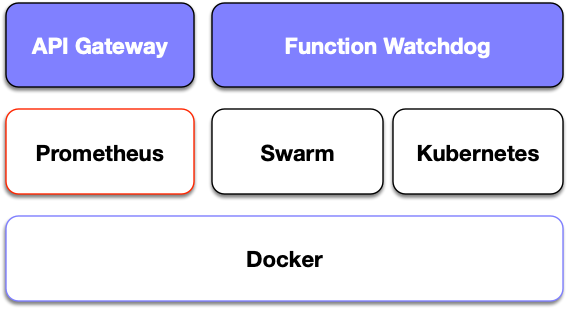
\includegraphics[width=0.8\textwidth]{img/openfaas-architectuur.png}
    \caption{Conceptuele voorstelling van de architectuur en componenten van OpenFaaS.}
    \label{fig:open-faas-conceptueel}  
\end{figure}

\begin{description}[style=unboxed, labelwidth=\linewidth, listparindent =0pt]
    \item[Docker laag]
    In figuur \ref{fig:open-faas-conceptueel} is de onderste laag een volledige Docker laag, dit weergeeft dat alle functies die geschreven worden, worden uitgevoerd in Docker containers. Deze containers bevatten alle dependencies nodig voor de code om uit te voeren.
    \\
    
    \item[Swarm/Kubernetes]
    Bovenop de Docker laag in figuur \ref{fig:open-faas-conceptueel} is er een Swarm of Kubernetes component terug te vinden. Deze laag is de zogenoemde ''orkestrator'', deze staat in voor het management, configuratie en de coördinatie van de Docker containers.
    \\
    
    \item[Prometheus]
    OpenFaaS maakt gebruik van Prometheus\footnote{https://prometheus.io/}, dit is een open source tool die instaat voor systeem monitoring en alerting. Prometheus verzamelt gegevens over de functies die kunnen worden weergegeven in een UI, namelijk Grafana dashboard.
    \\
    
    \item[Function Watchdog]
    In figuur \ref{fig:open-faas-conceptueel} staat de Function Watchdog bovenop de reeds opgesomde componenten. Function Watchdog zorgt ervoor dat een Docker image kan worden omgevormd in een serverless functie, dit door het toevoegen van een kleine HTTP server. Daarnaast is de Function Watchdog eveneens het ingangspunt dat HTTP requests toelaat om geforward te worden naar het bestemmingsproces via HTTP of STDIN. Het responsbericht wordt teruggestuurd naar STDOUT of HTTP van de applicatie. \autocite{Ellis2019}
    \newline
    
    \item[API Gateway/UI Portal]
    De API Gateway in figuur \ref{fig:open-faas-conceptueel} verzorgt een route naar de geschreven functies, hier worden functies gedefinieerd, en verzameld metrics aan de hand van Prometheus. De API Gateway zorgt eveneens voor schaalbaarheid van functies door de vraag op te halen via de replica count in Docker Swarm of de Kubernetes API. Bij installatie van OpenFaaS wordt er ook een UI meegeleverd, deze laat gebruikers toe functies op te vragen en toe te voegen via deze interface. \autocite{Ellis2019} 
    \\
    
    \item[CLI]
    Elk proces binnen een container of de container op zich kan een serverless functie zijn. OpenFaaS voorziet FaaS CLI om snel functies te deployen. Nieuwe functies kunnen worden gemaakt aan de hand van templates maar ook via een Dockerfile. \autocite{Ellis2019}  
\end{description}

\subsection{Fission}
Fission\footnote{https://fission.io} is een framework voor serverless functies op Kubernetes dat werd aangegeven door Nubera zelf, na verder onderzoek bleek dit ook te voldoen aan alle opgestelde requirements. Fission bestaat sinds augustus 2016 en wordt ontwikkeld en onderhouden door medewerkers van Platform9. Momenteel Heeft Fission vierduizend stars op GitHub en 76 contributors. Gebruikers die Fission reeds in hun organisatie implementeren zijn eveneens een stuk moeilijker te vinden in vergelijking met OpenFaaS gebruikers.
\\
De  belangrijkste aspecten van Fission zijn:
\begin{itemize}
    \item Native Kubernetes: Fission draait op elke locatie op Kubernetes.
    \item Snelle cold-start: functies hebben een korte cold-start latency, lager dan ~100ms.
    \item Functie samenstelling: Fission Workflows zorgt ervoor dat ontwikkelaars niet moeten bezig zijn met networking, bericht wachtrijen of andere onderdelen die serverless functies complex maken.
    \item Administratie en operationele eenvoud: logs worden onmiddellijk via de CLI weergegeven daarnaast is er ook integratie met Prometheus voor het evalueren van metrics aan de hand van een duidelijk dashboard.
    \item Istio integratie: Fission integreert met Istio, een platform dat instaat voor management en beveiliging van microservices. Via dashboards kunnen gebruikers ook informatie ophalen over de latency van functies die worden aangeroepen.
    \item Declaratie van functies moet maar éénmaal door de ontwikkelaar worden gedaan, vervolgens kan de functie overal worden gedeployed.
    \item Ondersteuning voor meerdere programmeertalen: Python, Node.js, GO, C\#, PHP daarnaast kunnen ook eigen containers worden gebouwd indien dit nodig is. 
    \item Auto-scaling van functies. 
\end{itemize}

\subsubsection{Architectuur}
Fission bestaat uit verschillende componenten, met elk hun eigen verantwoordelijkheden. Hieronder wordt een overzicht gegeven hoe een Fission architectuur precies in elkaar zit. 

\begin{figure}
    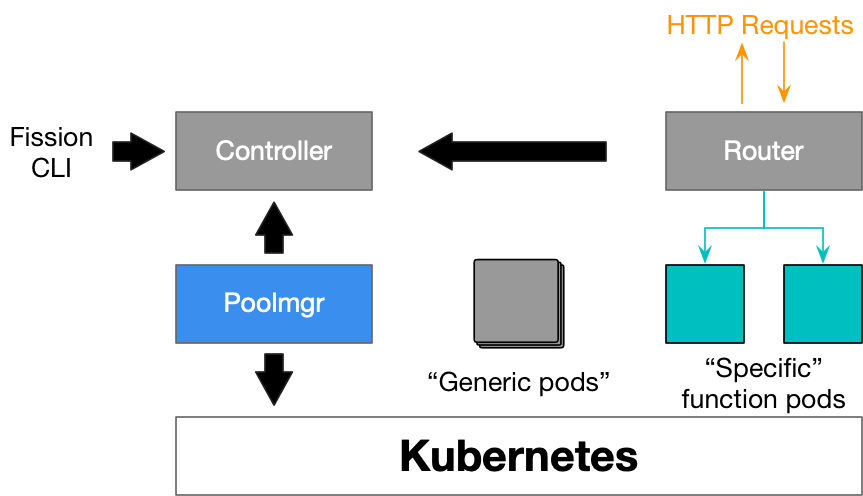
\includegraphics[width=0.9\textwidth]{img/fission-architectuur.png}
    \centering
    \caption{Architectuur van een het Fission framework dat draait bovenop een Kubernetes cluster. \autocite{Chemitiganti2018}}
    \label{fig:fission-architectuur}
\end{figure}

\begin{enumerate}
    \item Fission bestaat uit verschillende microservices. De controller houdt functies, event triggers, HTTP routes en omgevingsimages bij. Een pool manager (poolmgr) staat in voor het beheer van een groep omgevingscontainers (environment containers) die niet aan het werken zijn (geen functies uitvoeren). Daarnaast is de poolmgr ook verantwoordelijk voor het inladen van de functies in deze containers en na afloop de containers op te kuisen en ze weer naar initiële toestand te brengen. De router ontvangt, zoals te zien is in figuur \ref{fig:fission-architectuur} HTTP requests en routeert deze naar draaiende containers die de corresponderende functie bevatten, indien de nodige functie niet beschikbaar is wordt deze via de pool manager aangevraagd. \autocite{Chemitiganti2018}
    \item De controller bedient de Fission API terwijl alle andere componenten de controller in het oog houden voor updates. De router component wordt geëxposed als een Kubernetes dienst van de load balancer of NodePort type, dit afhankelijk van de locatie waar de cluster wordt gehost. Wanneer de router een HTTP request ontvangt kijkt hij eerst of er in de cache reeds een service is die gelinkt is met de request, zo niet zoekt hij de overeenstemmende functie om de request mee te mappen en vraagt hij de poolmgr voor een instantie. De poolmgr beschikt over een pool van pods die momenteel niet aan het werk zijn, de poolmgr kiest een pod waarin de functie wordt ingeladen. Als de functie is ingeladen wordt het adres van die pod teruggestuurd naar de router. De pod wordt nu opgeslagen in de cache voor toekomstige requests, indien er binnen enkele minuten geen nieuwe requests volgen wordt de pod gestopt.  \autocite{Chemitiganti2018}
    \item Fission voorziet een eenvoudige manier van functie deployment op Kubernetes clusters. Functies worden uitgevoerd los van elkaar.
    \item Voor het maken van complexere serverless applicaties moeten functies met elkaar kunnen communiceren en van elkaar gebruikmaken. Dit proces is vaak moeilijk en neemt veel tijd in beslag. Fission Workflows voorziet makkelijke orkestratie van een sequentie serverless functies voor het maken van een applicatie. \autocite{Chemitiganti2018}
    \item Workflows voorziet een makkelijke manier om serverless functies op elkaar af te stemmen en samen te laten werken aan de hand van sequenties van taken, conditionals en loops. Functies kunnen uitgevoerd worden om de beurt of parallel, daarnaast kan de output van een functie de input zijn van een andere. \autocite{Chemitiganti2018}
    \item In Fission worden logs bijgehouden in een databank aan de hand van Fluentd\footnote{https://www.fluentd.org/} en InfluxDB\footnote{https://www.influxdata.com/}. Logs kunnen worden opgevraagd via de CLI die Fission aanlevert.
    \item Monitoring van de infrastructuur is voorzien aan de hand van Prometheus.Via Prometheus worden metrics voor functies, zoals het aantal keer dat een functie wordt aangeroepen, het aantal errors, aanroeptijd, responstijd, cold starts, levensduur van een functie etc. gemeten.
\end{enumerate}

\subsubsection{Concepten}
\begin{description}[style=unboxed, labelwidth=\linewidth, listparindent =0pt]
    \item[Functie]
    Een functie is een stuk code, geschreven in een specifieke programmeertaal, dat wordt uitgevoerd wanneer deze wordt aangeroepen. Functies worden aangeroepen via requests die worden ontvangen op de Fission router. \autocite{Fission2018}
    \\
    
    \item[Environment]
    De environment container is specifiek per programmeertaal, deze voert de functie uit als respons op een HTTP request. Wanneer de Fission router een request ontvangt dan zal de environment container de functie in de runtime container inladen vervolgens wordt de functie uitgevoerd overeenkomstig met de request. \autocite{Fission2018}
    \\
    
    \item[Trigger]
    Een Fission object mapt requests aan functies in de backend. Wanneer een trigger een request ontvangt, wordt de doelfunctie gemapt aan de trigger aangeroepen via een HTTP request naar de Fission router. De router vraagt de functie in een pod eveneens op via een HTTP request. \autocite{Fission2018}
    \\
\end{description}


\subsubsection{Functie executors}
\label{sec:fission-executors}
\begin{description}[style=unboxed, labelwidth=\linewidth, listparindent =0pt]
    \item[Pool-based executor]
    De documentatie van \textcite{Fission2019} beschrijft een pool-based executor als volgt:
    Een pool-based executor (of Poolmgr) maakt een pool van generieke environment pods vanaf het moment dat een environment wordt aangemaakt. Op voorhand kan de gebruiker het aantal ''warme'' containers configureren, dit zijn een enkele environment containers die blijven draaien. De environment containers beschikken over functionaliteit die toelaat functies in te laden. Resource instellingen worden geconfigureerd op niveau van environment en worden door de functie pods geërfd. Wanneer een functie wordt aangemaakt en vervolgens aangeroepen, wordt een van de pods uit de pool van ''warme containers'' genomen en aangepast zodat deze kan gebruikt worden voor het uitvoeren van de functie. De pod die werd geoptimaliseerd wordt nu gebruikt voor het uitvoeren van de functie. Indien de pod na verloop van tijd geen requests meer ontvangt, dan zal Fission deze pod opruimen. Als er opnieuw reqests worden ontvangen nadat de pod werd opgeruimd dan wordt er weer een nieuwe pod geïnstantieerd en wordt deze gebruikt voor het uitvoeren van de functie. Pool-based executor type is interessant als functies een lage latency verwachten, daarentegen is het wel niet auto-scalable op basis van requests.
    \\
    
    \item[New-deployment executor]
    Een new-deployment executor of kortweg Newdeploy maakt een Kubernetes Deployment samen met een Service en HorizontalPodScaler(HPA) voor het uitvoeren van functies. Newdeploy maakt autoscaling en load balancing tussen pods mogelijk. Resource instellingen voor Newdeploys worden geconfigureerd op functie niveau, deze instellingen overschrijven de instellingen die gedefinieerd werden op environment niveau. New-deployment executors kunnen worden gebruikt voor functies die geen lage latency requirement hebben. De ''minscale'' waarde die definieert hoeveel deployments er van de functie standaard moeten draaien kan op nul worden ingesteld, bij aanroep van de functie zal Kubernetes dus een nieuwe Deployment met bijbehorende objecten aanmaken. Requests voor dezelfde functie binnen een bepaalde tijdspanne worden uitgevoerd door dezelfde deployment. Indien de functie voor een bepaalde tijd geen nieuwe requests ontvangt, dan zullen de objecten worden opgeruimd. Het Newdeploy mechanisme zorgt ervoor dat resource verbruik wordt gelimiteerd in overeenstemming met de requests die worden ontvangen.
    
    
    Functies waar er geen latency mag optreden kunnen eveneens gebruikmaken van de Newdeploy executor. Fission stelt gebruikers in staat om ''minscale'' op een waarde in te stellen hoger dan nul. het verhogen van de waarde zorgt ervoor dat er een minimum aantal pods draait wanneer er een functie wordt aangemaakt. Wanneer de functie in dit geval wordt aangeroepen dan zal er geen vertraging optreden omdat de pod waarin de functie draait reeds bestaat. Minscale zorgt er eveneens voor dat pods niet worden opgeruimd wanneer de functie voor een lange tijd niet wordt aangeroepen.
    \autocite{Fission2019}
    \\
    
    \item[Autoscaling]
    De Newdeploy executor voorziet autoscaling voor functies, dit gebaseerd op het verbruik van CPU. Gebruikers kunnen de standaard en maximum CPU voor een functie instellen evenals het CPU verbruik waarbij de autoscaling zal getriggerd worden. \autocite{Fission2019}
    \\
\end{description}

\subsection{Verschillen en overweging}
Tijdens de uitwerking van de shortlist werd duidelijk dat er over het ene framework meer terug te vinden is dan over het andere. De meeste documentatie en voorbeelden werden teruggevonden bij het zoeken naar OpenFaaS. In vergelijking met Fission is OpenFaaS op dit moment ook een stuk populairder en naar eigen mening ook duidelijker beschreven. Beide frameworks beschikken over een mooie documentatiewebsite, al is de website van OpenFaaS wel iets uitgebreider en duidelijker beschreven. Het is voor beginners ook makkelijker om in serverless te stappen met het OpenFaaS in vergelijking met Fission net omdat de documentatie hierover duidelijker is en aangenamer leest. OpenFaaS beschikt in tegenstelling tot Fission over meer relevante ''talks'' op YouTube en andere blog platformen. OpenFaaS pakt daarnaast ook uit met de eenvoud van installatie en garanderen een installatie die makkelijk uit te voeren is. Op basis van de ervaring opgedaan tijdens het onderzoek in deze short list lijkt OpenFaaS een zeer interessant alternatief voor Fission. In volgend hoofdstuk wordt er een Proof of Concept (PoC) opgezet van beide frameworks, op basis van deze PoC worden de requirements die nog niet gemeten werden vergeleken. Op basis van de Proof of Concept moet ook duidelijk zijn welk framework het interessantst zou kunnen zijn voor Nubera. De verschillen, gelijkenissen voor- en nadelen tussen Fission en OpenFaaS worden vergeleken.